\documentclass[12pt]{report}
\usepackage[a4paper,left=25.4mm, right=25.4mm, top=25.4mm, bottom=25.4mm]{geometry}
\usepackage[utf8]{inputenc}
\usepackage{graphicx}

%titlesec and titleformat for chapters without 'chapter 1' tags
\usepackage{titlesec} 
\titleformat{\chapter}[display]
  {\normalfont\bfseries}{}{0pt}{\Huge}

%for clickable table of contents
\usepackage{hyperref}
\hypersetup{
    colorlinks,
    citecolor=black,
    filecolor=black,
    linkcolor=black,
    urlcolor=black
}

%for glossary of terms
\usepackage[acronym]{glossaries}
\makeglossaries
\newacronym{cups}{CUPS}{Common Unix Printing System}

\graphicspath{ {img/} }
\title{
	{Thesis Title}\\
	{\large Universitatea Politehnica Timișoara}\\
	{
\includegraphics[width=50mm]{upt_logo.png}}
}
\author{Andrei Buruntia \\ andreiburuntia@gmail.com\\[1cm]{ Advisor: conf. dr. ing. Dan Cosma}}
\date{20-02-2018}
\begin{document}

\maketitle
\chapter*{Abstract}
În zilele noastre există o multitudine de imprimante și soluții de printing disponibile, fiecare cu interfața și setul ei de funcționalități. Această teză urmărește construirea unei platforme universale care să permită ascunderea imprimantelor după un strat de abstractizare suplimentar, oferind o singură interfață și posibilitatea de a furniza unei companii de printing date relevante sub formă de grafice.

Adresarea problemei anterior menționată necesită depășirea anumitor obstacole, trei dintre care fiind: abstractizarea imprimantei și a funcțiilor ei, integrarea imprimantelor moderne de orice fel, realizarea unor rapoarte închegate și coerente cu date extrase din procesul de printare, care să prezinte relevanță pentru utilizator, ideal permițând utilizatorului sa își creeze propria interfață, dupa nevoile și preferințele lui.

În consecință, lucrarea mea propune o soluție bazată pe \acrshort{cups}, care se ocupă de comunicațiile și controlul imprimantelor și de expunerea lor pe rețea. Acest lucru permite acoperirea unei game largi de imprimante, pastrearea complexității la un nivel relativ redus și accesarea informațiilor lower-level.

S-a considerat prioritară creerea unei platforme cap-coadă care sa nu restricționeze in vreun fel workflow-ul normal al unui utilizator.

Lucrarea arată potențialul folosirii tehnologiilor și sistemelor open-source la rezolvarea problemelor din ecosistemul corporate prin modificări si îmbunatațiri aduse acestora.

\chapter*{Ackowledgements}

\tableofcontents

\newpage

\chapter{Introducere}

	\section{Context și motivație}
Océ, compania in care lucrez, activeaza in domeniul de printing, fiind subsidiar Canon. In companie se pune problema analizei si colectarii datelor din procesul de imprimare. La propunerea companiei, am incercat sa abordez aceasta problema. Mai jos este prezentata mai pe larg problema, iar lucrarea urmareste propunerea unei idei de implementare a unu sistem care sa o rezolve. In aceasta documentatie se va incerca detalierea asupra anumitor aspecte ale lucrarii: dificultatile intalnite, probleme de comunicare, constraint-uri de orice fel, etc.

	\section[Problema.Analiza si colectare de statistici despre procesul de imprimare]{Problema \\ {\large Analiza si colectare de statistici despre procesul de imprimare}}

Pentru a putea optimiza costurile si procedeele de tiparire in cazul imprimamtelor de format mare se doreste analiza si colectarea de statistici referitoare la: 
\begin{enumerate}
\item Cantitatea de cerneala folosita
\item Tipul de material pe care se face tiparire
\item Informatii despre tipul de culoare 
\item Informatii despre metoda de finisare (capsare, copertare, lacuire. etc)
\end{enumerate}
Aceste informatii trebuiesc agregate si afisate sub forma unor grafice care pot fi folosite de catre utilizatori cat si de catre compania Océ. Utilizatorii vor avea informatii legate de costuri si timpi de executie. Compania Océ poate folosi aceste informatii in mod anonimizat pentru a culege informatii legate de calitatea tiparirii sia a procesului cat si pentru an analiza in mod proactiv procesul de tiparire si a colecta informatii despre modul in care imprimantele se comporta in timp si a preintamppina anumite defectiuni. 
Deoarece baza de imprimante este relative mare si nu toate imprimantele ofera in mod nativ informatii despre consumabilele si cantitatea de cerneala folosita se doreste ca aceste informatii sa fie colectate in mod transparent si de la imprimantele mai putin evaluate. Pentru aceasta ar trebui ca aceste informatii sa fie colectate intr-un mod cat mai transparent, fara a afecta functionarea normal a imprimantei si fara a afecta firmware-ul deja instalat. 
Informatiile astfel colectate  vor fi afisate intr-o interfata web accesibila utilizatorilor final si/sau ompaniei Océ. In ace4asta interfata grafica se vor afisa graficele necesare si se vor putea crea panouri de control dedicate.
Solutia trebuie sa fie extensibila, sa scaleze pe mai multe tipuiri de imprimanta. 
In cazul in care anumite informatii nu pot fi obtinute in mod direct din imprimanta atunci acestea trebuie sa poata fi generate prin analiza formatelor intermediare de tip rastru pe care rasterizatoarele le trimit catre imprimante. 
Implementarea solutiei trebuie sa respecte urmatoarele cerinte:
\begin{enumerate}
\item Sa nu expuna nicio informatie proprietara Océ
\item Se fie facuta intr-un limbaj de nivel inalt
\item Sa permita extensii cu costuri minime pentru modelele viitoare de imprimante
\item Sa implice  modificari minime la nivelul infrastructurii clentilor
\item Sa anonimizeze informatiile confidentiale 
\end{enumerate}

	\section{Descrierea proiectului}



\chapter{Fundamentare teoretică}


\chapter{Specificațiile proiectului}


\chapter{Design și implementare}

	\section{Arhitectură high-level}
		\begin{center}
			{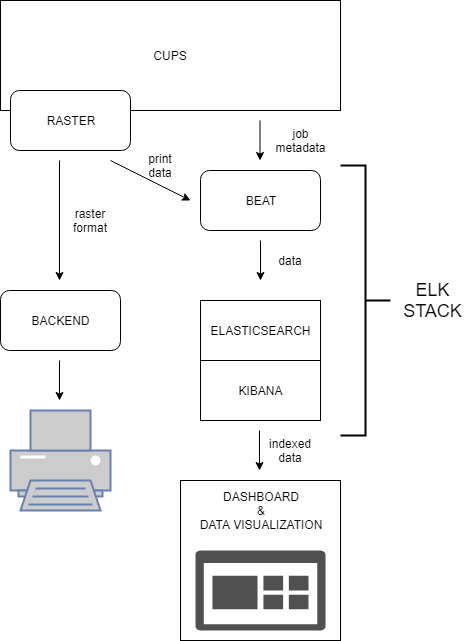
\includegraphics[width=110mm]{cups-arch.png}}
		\end{center}
		\subsection[CUPS]{CUPS\\ {\normalsize Common UNIX Printing System}}
Aparut in 1999, CUPS este un sistem modular de printing open-source pentru sistemele de operare Unix-like. Acesta permite unui calculator sa se comporte ca un print server, devenind un host care accepta job-uri de la clienti, le proceseaza si le trimite catre imprimante.
CUPS este format dintr-un spooler, un scheduler, un sistem de filtre care transforma datele dintr-un format in altul, si un sistem de backend-uri care realizeaza comunicarea cu imprimantele.

Workflow-ul standard CUPS este urmatorul: un job ajunge in scheduler, acesta il trimite catre unul sau mai multe filtre spre a fi convertit in alt format, apoi datele ajung intr-un backend de unde sunt trimise spre printer. Sistemul foloseste extensiv PostScript si rasterizarea datelor ca formate intelese de imprimante.
			\subsubsection{Scheduler-ul CUPS}
Scheduler-ul CUPS implementeaza Internet Printing Protocol si ofera o interfata web-based pentru managementul imprimantelor, job-urilor, configuratii server si documentatie. Pentru accesarea functionalitatilor de management si configuratie, un utilizator trebuie sa se autentifice. 
O alta parte foarte importanta a scheduler-ului este modulul de logging. Acesta inregistreaza evenimente legate de acces, erori sau page log.
Alte module importante ale schedeuler-ului sunt: modulul MIME (multipurpose internet mail extensions), modulul PPD (PostScript printer description), modulul care se ocupa cu management-ul dispozitivelor disponibile in sistem.


			\subsubsection{Sistemul de filtre CUPS}
Sistemul de filtre al CUPS poate procesa o varietate de formate. Acesta converteste datele unui print-job intr-un limbaj/format final printr-un sistem de filtre, folosind MIME types pentru identificarea formatelor.
Procesul de filtrare incepe prin determinarea tipului de date de intrare, folosind MIME databases. Printre filtrele default ale CUPS se numara: raster to PCL, raster to ESC/P, raster to Dymo, raster to ZPL.
Initial, am incercat modificare scheduler-ului, mai exact a modulului de logging, dar informatiile pe care le puteam obtine din acesta erau insuficiente pentru cerintele proiectului, in modulul de logging fiind expuse numai date despre utlizatori, job-uri sau status. Considerand nevoia de a obtine date despre pixeli, culoare, media, pagina, etc. s-a facut necesara accesarea informatiilor disponibile in sistem de filtre al CUPS, mai exact in unitatea de raster. Dupa ce am identificat informatiile de care am nevoie, le-am trimis catre exterior printr-un HTTP POST, apoi printr-un named pipe. Folosind un apel de sistem catre comanda cURL pentru a trimite cererea HTTP catre Beat, s-ar fi creat un numar de procese greu de controlat si care ar fi generat overhead pe care il puteam evita. O a doua alternativa ar fi fost folosirea unei biblioteci, de exemplu libcurl, pentru a inlocui apelurile de sistem, dar aceasta alternativa ar fi introdus o dependenta suplimentara in CUPS, ceea ce ar fi facut codul mai putin portabil si ar fi incalcat una din cerintele initiale ale proiectului. In final, am folosit un named pipe pentru transmiterea datelor, acesta fiind usor de accesat si generand overhead minim, iar in plus, datele nu sunt expuse in retea, aceasta interfata rezidand in kernelul sistemului de operare.


			\subsubsection{Backend-urile CUPS}
Backend-urile CUPS sunt folosite pentru a trimite datele catre imprimante. CUPS pune la dispozitie multe backend-uri: paralel, serial, USB, cups-pdf, PDF virtual printing, JetDirect, LPD, SMB, etc.
		
		
		\subsection[Elastic Stack]{Elastic Stack\\ {\normalsize Beater - Elasticsearch - Kibana}}
Elastic Stack este o stiva de aplicatii care permite extragerea, procesarea si vizualizarea datelor. In majoritatea cazurilor, acesta este gasit sub numele de ELK Stack (Elasticsearch - Logstash - Kibana). Pentru aceasta teza nu a fost folosit Logstash, fiind inlocuit cu un Elastic Beater ca unealta de colectare a datelor. Un Beat implementeaza interfata Beater si aduna date spre a le trimite catre Kibana sau, in cazul de fata, Elasticsearch.


			\subsubsection{Beat}
Beat-urile au fost adaugate recent la stack-ul ELK. Un Beat are responsabilitatea sa colecteze date si sa le trimita spre procesare sau vizualizare. Acesta trebuie sa implementeze in Golang o interfata numita Beater interface, care contine metode de Start, Run si Stop. Aceasta lucrare foloseste un Beat pentru a primi date de la raster-ul, raster care face parte din sistemul de filtre mentionat anterior. Beat-ul primeste raster data, face operatii de procesare si sanitization minimale, apoi trimite datele catre Elasticsearch. In implementarile conventionale de Beat, datele sunt transimse la intervale periodice de timp catre Elasticsearch sau Kibana. Implementarea Beat-ului din aceasta lucrare trimite date catre Elasticsearch atunci cand primeste informatii noi de la raster. cBeat (Beater-ul implementat pentru aceasta lucrare) urmatoarele componente principale:
\begin{enumerate}
\item {\large Metodele interfetei Beater}
	\subitem
	\textbf{metoda Run}
		\subsubitem contine bucla principala a aplicatiei
		\subsubitem in interiorul buclei se transmit evenimente catre restul ELK stack
		\subsubitem	un eveniment este trimis encodat ca JSON catre Elasticsearch


	\subitem
	\textbf{metoda Stop}
		\subsubitem este chemata atunci cand Beat-ul e semnalat sa se opreasca
\item  {\large Receptionarea datelor din CUPS}
	\subitem citirea din named pipe a evenimentelor se face prin deschiderea FIFO-ului ca orice alt fisier de pe disk, folosind modulul os al Golang
	\subitem FIFO-ului i s-a adaugat un mecanism de watch care ne notifica atunci cand s-a efectuat orice scriere in pipe
	\subitem functia care supravegheaza pipe-ul a fost lansata intr-o go rutina in metoda Run
	\subitem ca mecanism IPC s-a folosit un go channel intre green thread-ul care citeste din pipe si cel al metodei principale

\item {\large 
\end{enumerate}


			\subsubsection{Elasticsearch}
Elasticsearch este un motor de cautare bazat pe Apache Lucene. Ofer clienti disponibili in majoritatea tehnologiilor si este cel mai popular motor de cautare enterprise. Beneficiile Elasticsearch includ: cautare foarte scalabila, aproape real-time, suportul mai multor clienti, platforma distribuita. Este considerat de multi backbone-ul stack-ului ELK. Informatiile extrase de Beat ajung in Elasticsearch, iar acesta cauta tipare si indexeaza datele spre a le trimite catre Kibana.


			\subsubsection{Kibana}
Kibana este un plugin open source pentru vizualizare de data, care pune la dispozitie capabilitati de vizualizare ale elementelor indexate intr-un cluster Elasticsearch. Un utilizator poate  construi diferite tipuri de grafice bazate pe datele indexate de Elasticsearch, iar pe baza acestor grafice se pot construi dashboard-uri configurabile. Kibana preia datele indexat de la Elastisearch si le foloseste la generarea de grafice si vizualizari relevante pentru utilizator.


	\section{Comunicarea între module}

\chapter{Rezultate}

\chapter{Concluzii}

\chapter{References}

\chapter{Glosar de termeni}
\acrshort{cups} - \acrlong{cups}
PDF - 

\clearpage

\printglossaries
\end{document}
